\documentclass[tikz,border=3mm]{standalone}

\usepackage[scaled]{helvet}
\renewcommand{\familydefault}{\sfdefault} % Setzt die Standardschriftart auf sans-serif

\usepackage{tikz}
\usetikzlibrary{
    shapes.geometric,
    arrows.meta,
    positioning,
    fit,
    backgrounds
}

\usepackage{flowchart}

\tikzset{
    endpoint/.style={
        draw,
        rectangle,
        rounded corners=2mm,
        minimum width=2.5cm,
        minimum height=0.8cm,
        align=center,
        fill=green!15  
    },
    process/.style={
        draw,
        rectangle,
        rounded corners,
        minimum width=2.5cm,
        minimum height=0.8cm,
        align=center,
        fill=violet!15
    },
    decision/.style={
        draw,
        diamond,
        aspect=2,
        minimum width=3cm,
        align=center,
        fill=yellow!20
    },
    helper/.style={
        draw,
        rectangle,
        rounded corners,
        minimum width=2.5cm,
        minimum height=0.8cm,
        align=center,
        fill=cyan!15
    },
    predefined process/.style={  % Note the space in the name
        % Basic shape and border
        draw,
        predproc,
        minimum width=2.5cm,
        align=center,
        fill=blue!10
    },
    arrow/.style={
        -Stealth,
        thick
    }
}

\begin{document}
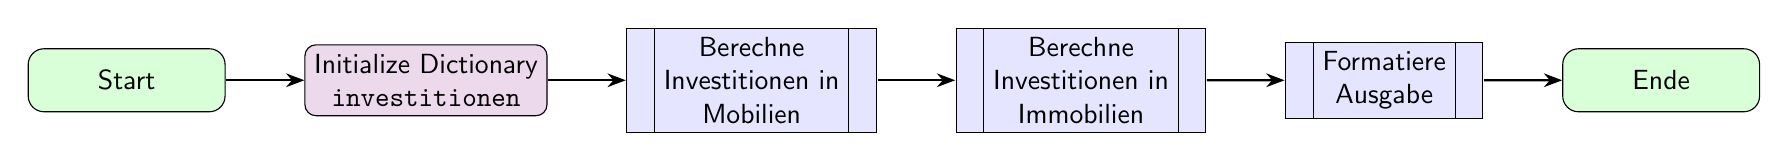
\begin{tikzpicture}
    \node[endpoint] (start) {Start};
    \node[process, right=of start] (init) {Initialize Dictionary \\
    \texttt{investitionen}};
    \node[predefined process, right=of init] (mob) {Berechne \\ Investitionen in
    \\ Mobilien};
    \node[predefined process, right=of mob] (imm) {Berechne \\ Investitionen in
    \\ Immobilien};
    \node[predefined process, right=of imm] (form) {Formatiere \\ Ausgabe};
    \node[endpoint, right=of form] (end) {Ende};

    \draw[arrow] (start) -- (init);
    \draw[arrow] (init) -- (mob);
    \draw[arrow] (mob) -- (imm);
    \draw[arrow] (imm) -- (form);
    \draw[arrow] (form) -- (end);
    
\end{tikzpicture}
\end{document}